\documentclass[11pt,a4paper]{scrreprt}

\usepackage[utf8]{inputenc}
\usepackage[T1]{fontenc}
%\usepackage{scrpage2}
\usepackage{amssymb}
\usepackage{amsmath}
\usepackage[style=authoryear,backend=biber]{biblatex}
\usepackage{bm}
\usepackage{commath}
%\usepackage{booktabs}
%\usepackage[flushmargin,ragged]{footmisc}
\usepackage{graphicx}
%\usepackage{ifthen}
%\usepackage{lastpage}
\usepackage{nag}
%\usepackage{ngerman}
\usepackage{enumerate}
%\usepackage{hhline}
%\usepackage{listings}
%\usepackage{xr-hyper}
\usepackage{hyperref}
%\usepackage{units}
\usepackage{upgreek}
%\usepackage{xcolor}

%\lstset{basicstyle=\fontfamily{pcr}\selectfont, keywordstyle=\bfseries, language=C++}
\newcommand{\vc}[1]{\bm{#1}}
\newcommand{\vcc}[1]{\textbf{#1}}
\newcommand{\mat}[1]{\bm{#1}}
\newcommand{\T}{^{\top}}
\newcommand{\e}{\mathrm e}
\DeclareMathOperator*{\argmax}{argmax}
\DeclareMathOperator{\cov}{cov}
\DeclareMathOperator{\diag}{diag}
\DeclareMathOperator*{\mslim}{mslim}

\newcommand{\newterm}[1]{\emph{#1}}

\addbibresource{references.bib}

\title{Gaussian Processes for Plume Distribution Estimation with UAVs}
\author{Jan Gosmann}
\makeatletter
% FIXME
%\hypersetup{
  %pdftitle={\@title},
  %pdfauthor={\@author},
  %pdfsubject={},
  %pdfkeywords={}
%}
\makeatother

\begin{document}
\maketitle

\chapter{Introduction}
Environmental monitoring is important in various ways. It is needed to ensure 
water and air pollution levels are in compliance with regulations like 
\textcite{Anonymous:1996ui}, to monitor ozone concentrations and climate change,  
as well as surveillance of industrial facilities for leakages of pollutants to 
just name a few applications.

In many of these scenarios it is feasible to have a static sensor network and 
there is already existing research on how to optimally utilize sensors at fixed 
locations \parencite[e.g.][]{Osborne:2008hi, Guestrin:2005cq, Wang:kz}.  
However, better results may be obtainable using mobile robots which can move to 
and acquire more precise data in interesting areas. Moreover, in some scenarios 
like disaster response where timely information is needed it might not be 
possible to first deploy an extensive sensor network. Mobile robots allow here 
to quickly identify the interesting regions and gather data primarily in those.  
The problem of autonomously choosing the interesting locations for data 
acquisition is known as \newterm{active learning}. \textcite{Marchant:2012wb} 
also used the term \newterm{Intelligent Environmental Monitoring} (IEM) 

In this work I focus on a scenario proposed as part of the CompLACS project in 
\textcite{denardi2013rn}: One or more sources emit gaseous substance or aerosol 
which is dispersed by a constant wind. The resulting plume distribution has to 
be estimated with autonomously controlled unmanned aerial vehicles (UAVs). The 
rather steep concentration gradients and small spatial extend orthogonal to the 
dispersion direction especially add to the difficulty of this problem.  With few 
UAVs it is not possible to cover the whole volume of investigation densely 
enough using a regular pattern in a timely manner. It is necessary to focus 
measurement to specific areas. Furthermore, measurement noise has to be taken in 
consideration.

In previous work swarms of robots have been used to localize the source of 
a plume \parencite{Jatmiko:2007df, Zarzhitsky:2005tz}. These approaches, 
however, do not allow the usage of only one robot and do not provide one with an 
estimation of the plume dispersion. Such an estimation might be important for 
various reasons such as determining areas in which a threshold is exceeded or 
a contamination occurred. As \textcite{Reggente:2009ti} noted, though one could 
try to model the actual fluid dynamics to obtain these information, such 
computational fluid dynamics models become intractable for real world 
applications with inaccurate data.  Instead they propose to build a statistical 
model with the gas concentration measurements as random variables.

A widely used statistical model for spatial or spatio-temporal data are 
\newterm{Gaussian processes}\footnote{In geospatial statistics the modelling 
    with Gaussian processes is also known as \newterm{kriging}.}. In several 
works \parencite[e.g.][]{Stachniss:2008vz, Marchant:2012wb} the modelled data 
were actually gas concentrations. Also, there exists some prior work on actively 
selecting the sampling locations. \Textcite{Stranders:2008wl} do this for 
discrete locations; \textcite{Singh:2010wt} and \textcite{Marchant:2012wb} for 
continuous locations. However, none of these approaches is optimal for plume 
dispersions.

TODO overview over chapters

\chapter{Gaussian Processes}
A vast number of regression methods has been proposed in the machine learning 
literature. In this work I use Gaussian Processes as these have been 
successfully used in a number of studies related to environmental monitoring and 
modelling of gas distributions (TODO refs). Gaussian Processes exhibit a number 
of desirable features. They are non-parametric, non-linear and therefore do not 
require any assumptions about the underlying functions or limitations of the 
search space. Also, they provide one with an estimate of the predictive 
uncertainties which can be used for a natural exploration-exploitation 
trade-off.

In the remainder of the chapter I will discuss the essentials of Gaussian 
Process regression. A more thorough introduction can be found in 
\textcite{Rasmussen:2006vz}.

Let $\mathcal{D} = \{(\vc{x}_i, y_i) | i = 1, \dots, N\}$ a set of training data 
with inputs $\vc x$ and outputs $y = f(\vc x) + \eta$ with additive noise $\eta 
\sim \mathcal{N}(0, \sigma_{\text{n}}^2)$. We want to learn the function $f(\vc 
x)$ from this training data.

A Gaussian Process
\begin{equation}
    f(\vc x) \sim \mathcal{GP}(m(\vc x), k(\vc x, \vc x'))
\end{equation}
imposes a multivariate Gaussian distribution on the space of functions $f(\vc 
x)$. It is completely specified by the mean function $m(\vc x)$ and covariance 
function $k(\vc x, \vc x')$. Usually, though not necessary, the mean function is 
taken to be zero. In most scenarios the choice of the covariance function is 
much more interesting as it controls features like smoothness of the predicted 
underlying function. I will discuss this topic regarding the modelling problem 
on hand in chapter TODO.

We can now formulate the joint Gaussian prior distribution of the observed 
training targets and the predicted values $\vc f_*$ at unseen locations $X_*$ 
(assuming $m(\vc x) = 0$):
\begin{equation}
    \left[ \begin{array}{c}\vc y \\ \vc f_* \end{array} \right]
    \sim \mathcal{N}\left(\vc 0,
        \left[ \begin{array}{cc}
            K(X, X) + \sigma_{\text{n}}^2 \mat I & K(X, X_*) \\ K(X_*, X) 
            & K(X_*, X_*)
        \end{array} \right]
    \right)
\end{equation}
Here $K(X, X')$ are matrices with the elements $(i, j)$ being the covariances 
$k(\vc x_i, \vc x'_j)$ evaluated for all pairs $\vc x_i \in X$ and $\vc x'_j \in 
X'$. In the following I will use $\tilde{\mat K} = K(X, X) + \sigma_{\text{n}}^2 
\mat I$ as a shorter notation. By conditioning on the observations one obtains 
the predictive distribution for $\vc f_*$ as
\begin{align}
    \vc f_* | X, \vc y, X_* &\sim \mathcal{N}(\bar{\vc f_*}, \cov(\vc 
    f_*))\text{, with}\\
    \bar{\vc f_*} &= \mu(X_*) = K(X_*, X)\tilde{\mat K}^{-1} \vc y\text{,} \\
    \cov(\vc f_*) &= K(X_*, X_*) - K(X_*, X)\tilde{\mat K}^{-1}K(X, X_*) 
    \\
    \sigma^2(X_*) &= \diag(\cov(\vc f_*)) \text{.}
\end{align}

Even though, $K$ is a symmetric, positive-definite matrix it can be 
ill-conditioned.\footnote{The condition $\kappa(A)$ of a matrix $A$ is defined 
    as $\kappa(\mat A) = \|\mat A\| \|\mat A^{-1}\|$. Using the $L_2$-norm this 
    corresponds to $\kappa(\mat A) = \frac{\lambda_1}{\lambda_n}$,
    the ratio of the largest eigenvalue $\lambda_1$ and the smallest one
    $\lambda_n$. If the condition number $\kappa(\mat A)$ is too large, the 
    matrix is near-singular and ill-conditioned.} This happens especially for 
close-by input data points as they occur in a sequential scenario like the plume 
modelling here.

There are two commonly implemented approaches to counteract the problem of 
ill-conditioning \parencite[cp.]{Sacks:1989cv, Neal:1997tj, Booker:1999wz, 
    Gramacy:2008es}. Firstly, instead of using a general matrix inversion 
algorithm one can utilize the symmetry and positive-definiteness of $\tilde{\mat 
    K}$ by doing a Cholesky decomposition. That yields a lower, triangular 
matrix $L$ satisfying $\tilde{\mat K} = \mat L\mat L\T$. The inverse can the be 
calculated as $\tilde{\mat K}^{-1} = (\mat L^{-1})\T \mat L^{-1}$. Secondly, 
a well conditioned $\tilde{\mat K}$ can be ensured by adding a nugget $g > 0$ 
(also known as jitter) to the diagonal of the covariance matrix. This will 
increase all eigenvalues by the same value and thus improve the condition.  The 
addition of a nugget can also be seen as increasing the noise variance 
$\sigma_{\text{n}}^2$ and thus allowing the Gaussian Process to match the target 
less precisely and to become smoother.

% TODO some example images

\section{Online Updates}
A naive implementation requires a $O(N^3)$ matrix inversion whenever new data 
points are added to the Gaussian Process with $N$ being the total number of data 
points collected so far. However, it is possible to do online updates with $n 
< N$ new data points where only a $n \times n$ matrix has to be inverted. This 
reduces the complexity of the matrix inversion to $O(n^3)$ and the overall 
complexity including the necessary matrix multiplications to $O(n [\max\{n, 
N - n\}]^2)$.

Let us denote the set of inputs already trained on with $X$ and the set of 
inputs to add as $X'$. The block covariance matrix after adding these new inputs 
will be
\begin{equation} \label{eqn:tilde_K_prime}
    \tilde{\mat K}' = \left[ \begin{array}{cc}
            \tilde{\mat K} & K(X, X') \\ K(X', X) & K(X', X') 
            + \sigma_{\text{n}}^2\mat I
        \end{array}
    \right]\text{.}
\end{equation}
The Cholesky factorization can also be written with block matrices
\begin{equation}
    \tilde{\mat K}' = \mat L \mat L\T = \left[
        \begin{array}{cc}
            \mat A & \mat 0 \\ \mat B & \mat C
        \end{array}
    \right] \left[
        \begin{array}{cc}
            \mat A\T & \mat B\T \\ \mat 0 & \mat C\T
        \end{array}
    \right] = \left[
        \begin{array}{cc}
            \mat A \mat A\T & \mat A \mat B\T \\ \mat B \mat A\T & \mat B \mat 
            B\T + \mat C \mat C\T
        \end{array}
    \right]
\end{equation}
and comparison with equation~(\ref{eqn:tilde_K_prime}) gives the following 
relations:
FIXME: the L is used for two different sized matrices!
\begin{align}
    \mat A &= \mat L \\
    \mat B &= K(X', X) (\mat L\T)^{-1} \\
    \mat C \mat C\T &= K(X', X') + \sigma_{\text{n}}^2\mat I - K(X', 
    X)\tilde{\mat K}^{-1}K(X, X')
\end{align}
As $\mat C \mat C\T$ is symmetric, positive-definite it is possible to obtain 
$\mat C$ by a Cholesky decomposition.
With the inverse of a block matrix \parencite[45]{Petersen:2008wc} we obtain the 
following relation for the inverse of the updated Cholesky factor:
\begin{equation}
    \mat L' = \left[
        \begin{array}{cc}
            \mat L^{-1} & \mat 0 \\ -\mat C^{-1} K(X', X)\tilde{\mat K}^{-1} 
            & \mat C^{-1}
        \end{array}
    \right]
\end{equation}

\section{Sparse Approximations}

\section{Covariance Functions}
The choice of the covariance function determines the assumptions about the 
functions learned with a Gaussian process. Hence, it is quite important. In this 
chapter I will discuss some widely used covariance functions and considerations 
to take into account. A more thorough discussion including further covariance 
functions is to be found in \textcite[Chapter 4]{Rasmussen:2006vz} on which this 
section is based.

A valid covariance function $k(\vc x, \vc x')$ has to be semi-positive definite 
kernel \parencite{Cressie:1993uu} satisfying
\begin{equation}
    \int f(\vc x) k(\vc x, \vc x') f(\vc x') \dif \mu(\vc x) \dif \mu(\vc x') 
    \geq 0
\end{equation}
with $f \in L_2(\mathcal{X}, \mu)$. This ensures that the kernel's Gram matrix 
for a set of inputs $\cbr{x_i | i = 1, \dots, n}$ with entries $\mat K_{ij} 
= k(\vc x_i, \vc x_j)$ is also semi-positive definite and therefore a valid, 
invertible covariance matrix.

The choice of covariance function determines the smoothness of the Gaussian 
process. This is formalized in the notion of how many times it is \newterm{mean 
    square (MS) differentiable}. A process $f(\vc x)$ is differentiable if the
mean square limit denoted by $\mslim$ exists in the mean square derivative given 
by
\begin{equation}
    \dpd{f(\vc x)}{x_i} = \mslim_{h \rightarrow 0} \frac{f(\vc x + h\vcc e_i) 
    - f(\vc x)}{h}
\end{equation}
for the $i$-th direction with the unit vector $\vcc e_i$.

%defined in \textcite[81]{Rasmussen:2006vz} in the following way: ``Let $x_1, 
%x_2, \dots$ be a sequence of points and $x_*$ be a fixed point in $\mathbb{R}^D$ 
%such that $\abs{x_k - x_*} \rightarrow 0$ as $k \rightarrow \infty$. Then 
%a process $f(x)$ is continuous in mean square at $x_*$ if 
%$\mathbb{E}[\abs[0]{f(x_k) - f(x_*)}^2] \rightarrow 0$ as $k \rightarrow 
%\infty$. If this holds for all $x_* \in A$ where $A$ is a subset of 
%$\mathbb{R}^D$ then $f(x)$ is said to be continuous in mean square (MS) over 
%$A$.''

\subsection{Stationary Covariance Functions}
A kernel which is only a function of $\vc x - \vc x'$ is called 
\newterm{stationary} and is invariant to translations. Furthermore, it is 
\newterm{isotropic} if it is a radial basis function (RBF) $k(r)$ with $r 
= \abs{\vc x - \vc x'}$.  An isotropic kernel is invariant to all rigid motions.

For stationary kernels the smoothness properties of the resulting Gaussian 
process can be easily obtained: It is $k$-times differentiable if at $\vc 
x = \vc 0$ the $2k$-th order partial derivatives $\partial^{2k} k(\vc x) 
/ \partial x_{i_1}^2 \dots \partial x_{i_k}^2$ exist and are finite. Thus, the 
process smoothness is essentially determined by the kernel properties around 
$\vc 0$.

A common default choice is the \newterm{squared exponential} (SE) kernel defined 
as
\begin{equation}
    k_{\text{SE}}(r) = \sigma_k^2 \exp\del{-\frac{r^2}{-2\ell^2}}
\end{equation}
with the desired process variance $\sigma_k^2$ and length-scale $\ell$. It 
produces infinitely MS differentiable Gaussian processes. This can, actually, be 
too smooth in many applications.

The Mat\'ern class of covariance functions allows to control the smoothness with 
a parameter $\nu$. Using the modified Bessel function $K_{\nu}$ it is given by
\begin{equation}
    k_{\nu}(r) = \sigma_k^2 \frac{2^{1-\nu}}{\Gamma(\nu)} 
    \del{\frac{r\sqrt{2\nu}}{\ell}}^{\nu} K_{\nu} 
    \del{\frac{r\sqrt{2\nu}}{\ell}}
\end{equation}
The resulting Gaussian process will be $k$ times MS differentiable for $k 
< \nu$. The parameter $\ell$ denotes again the characteristic length-scale.

Typically, only the kernels with $2\nu \in \cbr{1, 2, 3}$ are used.  Usually the 
(noisy) data allows not to differentiate which kernel to use for larger $\nu$.  
Half-integer values are used as the kernel function will become quite simple:
\begin{align}
    k_{5/2}(r) &= \sigma_k^2 \del{1 + \frac{r\sqrt{5}}{\ell} 
        + \frac{5r^2}{3\ell^2}} \exp\del{-\frac{r\sqrt{5}}{\ell}} \\
    k_{3/2}(r) &= \sigma_k^2 \del{1 + \frac{r\sqrt{3}}{\ell}} 
    \exp\del{-\frac{r\sqrt{3}}{\ell}} \\
    k_{1/2}(r) &= k_{\exp}(r) = \sigma_k^2 \exp\del{-\frac{r}{\ell}}
\end{align}
From these kernel functions $k_{\nu=1/2}(r)$ is also known as the 
\newterm{exponential kernel}. Furthermore, note that for $\nu \rightarrow 
\infty$ the squared exponential kernel is recovered.

% TODO include MS continuity?

\subsection{Non-stationary Covariance Functions}
Many phenomena, including the concentrations of gas plumes, are not stationary.  
Already a (shifted) Gaussian density function exhibits different optimal 
length-scales (see TODO fig). The rate of change along the tails is low leading 
to a large length-scale, whereas around the mean the length-scale is much 
shorter.  Moreover, discontinuities at specific places can be easier modelled 
using non-stationary kernels.

However, the usage of non-stationary covariance functions for the given plume 
modelling problem is far from straight forward and might need more prior 
knowledge than one is willing to assume (in simulations) or effectively has.  
One would probably have to use different kernels depending on the scenario 
(wind/no wind, number of sources) and these would have to be parameterized with 
the source locations. Otherwise the non-stationarity of the kernel could not 
relate to the actual non-stationarity of the plume.

Methods for selecting such parameters will be discussed in the next section.  
Unfortunately, the cost of these methods grows with the number of parameters 
which for non-stationary kernels will be larger. Matters are complicated even 
more as it is usually desirable to have a differentiable kernel to be able to 
use gradient-based optimizers. In an active learning scenario, moreover, there 
is a limited amount of data in the beginning making the correct estimation of 
parameters like the source position virtually impossible.

TODO: read and maybe include non-stationary papers
TODO: non-stationary not agnostic to structure.

\section{Hyper-parameter Selection}
Though Gaussian processes are non-parametric, the choice of covariance function 
will introduce hyper-parameters $\vc \theta$ like the length-scale which have to 
be set.  In the following I will discuss three methods for doing so.

With the \newterm{test set method} all data available $\mathcal{D}$ will be 
split into two sets $\mathcal{D}_0$ and $\mathcal{D}_*$. The first one 
$\mathcal{D}_0$ is used to train Gaussian processes with different covariance 
functions and hyper-parameters. For each model the generalization error 
$E_{\text{G}}$ over the test set $\mathcal{D}_*$ will be evaluated and one 
choses the parameters with the minimal generalization error. The error measure 
can be chosen freely, with the root mean square error being a typical choice 
(see also section TODO).

If the amount of data available is low, it is common to use \newterm{$k$-fold 
    cross validation} where $\mathcal{D}$ is split into $k$ disjoint subsets 
$\mathcal{D}_i$ of equal size and the generalization error will be calculated 
from $k$ models using the respective $\mathcal{D}_i$ as test set and the other 
sets as training data.

The third possibility is to find $\argmax_{\vc \theta} p(\vc\theta | \vc y, \mat 
X, \mathcal{H}_i)$, wherein
\begin{equation}
    p(\vc\theta | \vc y, \mat X, \mathcal{H}_i) = \frac{p(\vc y | \mat X, 
        \vc\theta, \mathcal{H}_i) p(\vc\theta | \mathcal{H}_i)}{p(\vc y | \mat 
        X, \mathcal{H}_i)}
\end{equation}
with marginal likelihood $p(\vc y | \mat X, \vc\theta, \mathcal{H}_i)$, prior 
$p(\vc\theta | \mathcal{H}_i)$, normalization factor $p(\vc y | \mat X, 
\mathcal{H}_i)$, and a set of possible model structures $\mathcal{H}_i$. The 
normalization factor can be difficult to estimate 
\parencite[109]{Rasmussen:2006vz}. For that reason often, even thought it can 
more easily lead to overfitting, only the marginal likelihood is optimized which 
is known as type~II maximum likelihood. For a Gaussian process with $n$ training 
samples it is given by
\begin{equation}
    \log p(\vc y | \mat X, \vc\theta) = -\frac{1}{2}\del{\vc y\T \tilde{\mat 
            K}^{-1} \vc y + \log \det \tilde{\mat K} + n \log 2\uppi} \text{.}
\end{equation}
The three summands can be interpreted as the quality of the data fit $\vc y\T 
\tilde{\mat K}^{-1} \vc y$, model complexity $\log \det \tilde{\mat K}$, and 
a normalization term $n \log 2\uppi$. Hence, the optimization of the marginal 
likelihood includes an automatic trade-off of model complexity and data fit.

Optimizing the marginal likelihood has the advantage in comparison to the test 
set method that a gradient based optimizer can be used. The partial derivatives 
of the likelihood are given by
\begin{equation}
    \dpd{}{\theta_j} \log p(\vc y | \mat X, \vc\theta) = \frac{1}{2} 
    \del{\del{\tilde{\mat K}^{-1}\vc y \vc y\T \tilde{\mat K}^{-1} - \tilde{\mat 
                K}^{-1}} \dpd{\tilde{\mat K}}{\theta_j}} \text{.}
\end{equation}
However, all method require a complete retraining of the Gaussian process as for 
each update of the hyper-parameters $\tilde{\mat K}^{-1}$ has to be newly 
calculated. Thus, in an online setting it is far more efficient to keep the 
hyper-parameters fixed or only update them occasionally.

TODO: Gaussian Process Mixtures? Efficiency in case of parallel calculation?
How is the selection happening? Error or likelihood?

\section{Active Learning}
A setting in which a learning algorithm can freely choose the next training 
input is called \newterm{active learning}. A general introduction in the topic 
is provided by \textcite{Settles:2009vo}. Here, I will focus on how to realize 
active learning in the context of Gaussian processes.

In general, one defines a \newterm{utility} or \newterm{acquisition} function 
$u(\vc x)$ indicating the expected benefit for choosing $\vc x$ as next training 
sample. Hence, the optimal choice is $\argmax_{\vc x} u(\vc x)$. Equivalently, 
it is possible to use the negative of a loss function $u(\vc x) = - \lambda(\vc 
x)$.

The choice of $u(\vc x)$ influences the exploration-exploitation trade-off and 
on which areas of the input space the learning will be focussed. In the 
estimation of a plume distribution samples should be acquired mostly at places 
with high concentrations, but once such an area is well estimated further 
exploration should follow to possibly find further sources.

\Textcite{Marchant:2012wb} proposed the \newterm{distance-based upper confidence 
    bound} (DUCB) for a similar scenario of environmental monitoring where ozone 
concentrations over US territory were to be measured:
\begin{equation}
    u_{\text{DUCB}}(\vc x) = \mu(\vc x) + \kappa \cdot \sigma^2(\vc x) + \gamma 
    \cdot d(\vc x, \vc x')
\end{equation}
The mean prediction $\mu(\vc x)$ and the predictive variance $\sigma^2(\vc x)$ 
are obtained directly from the Gaussian process, $d(\vc x, \vc x')$ denotes the 
Euclidean distance of $\vc x$ to the last sample location $\vc x'$. The 
parameter $\kappa$ controls the exploration-exploitation balance. Higher values 
give more importance to decreasing the predictive variance and lead to more 
exploration. The parameter $\gamma \leq 0$ adjusts the distance penalty.  
Favoring location near to the current UAV position might decrease the distance 
travelled and save energy as well as time.

Though, the scenario above appears to be quite similar to the problem at hand 
one should note a certain difference. The ozone concentration is a quite smooth 
distribution as \textcite{Marchant:2012wb} used the squared exponential 
covariance function to obtain reasonable results. In opposite to that, the 
spatial distribution of a gas plume is much more localized \parencite[][this was 
also noted by]{Stachniss:2008vz}. Thus, I propose \newterm{plume distance-based 
    upper confidence bound} (PDUCB) acquisition function inspired by DUCB, but 
adjusted:
\begin{equation}
    u_{\text{PDUCB}}(\vc x) = \del{1 - a} \cdot \ln\del{\mu_+(\vc x) 
        + \varepsilon} + a \cdot \ln \varepsilon + \kappa \cdot \sigma^2(\vc x) 
    + \gamma \cdot d^2(\vc x, \vc x')
\end{equation}
with
\begin{align}
    a &= \e^{-\mu_+(\vc x) / \varepsilon} \\
    \mu_+(\vc x) &= \max\cbr{0, \mu(\vc x)}
\end{align}
Using the logarithm of the prediction mean makes this utility function sensitive 
for small concentrations which can hint towards areas with higher concentration.  
Being sensitive to the same absolute change for high concentrations is not as 
important. As the concentration might be equal to zero strict positiveness has 
to be explicitly ensured by a small $\varepsilon > 0$. The predictive standard 
deviation $\sigma(\vc x)$ in comparison to the variance $\sigma^2(\vc x)$ should 
put more weight on also reducing the uncertainty in areas where it is already 
reduced (but non-zero) instead of primarily focus on the areas with maximum 
uncertainty. Similarly, the squaring of the distance will reduce the penalty 
around $\vc x'$ (while increasing it further away). This should be advantageous 
as the unsquared distance function tends to force $\vc x$ much closer to $\vc 
x'$, but the next sample though it should be near to $\vc x'$ should not be too 
close to $\vc x'$. Otherwise, not much new information would be gained.

Apart from some explicit values, \textcite{Marchant:2012wb} do not discuss how 
to choose the parameters $\kappa$ and $\gamma$. Nevertheless, some observations 
can be made for both DUCB and PDUCB. Firstly, one should choose $\kappa \cdot 
\max \sigma^2(\vc x) > \max \mu(\vc x)$. Otherwise, one can get stuck in a local 
maximum as the mean prediction term might get larger than the predictive 
variance anywhere in the input space. Even though, it can be a good strategy to 
exploit maxima first exploration should continue once the distribution around 
the maximum is accurately known. A too large $\kappa$ is also problematic as it 
prevents any exploitation. Secondly, $\abs{\gamma}$ should not be too large or 
the distance penalty would dominate and also lead to one getting stuck in one 
position $\vc x = \vc x'$. Thirdly, $\varepsilon$ influences the sensitivity for 
low concentrations and should therefore be small, but large enough too prevent 
numerical problems in the evaluation of the logarithm. A value of $\varepsilon 
= 10^{-30}$ seems to work well (see section TODO).

Typically, one knows the spatial dimensions of the input space which allows to 
estimate a reasonable $\gamma$. However, the maximal $\vc y$ determining $\max 
\mu(\vc x)$ might not be known in advance. Thus, it would be helpful to set 
$\kappa$ automatically from $\vc y$, the data seen so far. This can be done by 
setting $\kappa = \kappa_{\text{DUCB}}(\vc y)$ (for DUCB) and $\kappa 
= \kappa_{\text{PDUCB}}(\vc y)$ (for PDUCB) respectively with
\begin{align}
    \kappa_{\text{DUCB}}(\vc y) &= \kappa' \cdot \max \vc y \\
    \kappa_{\text{PDUCB}}(\vc y) &= \kappa' \cdot \del{\ln(\max \vc 
        y + \varepsilon) - \ln \varepsilon}
\end{align}
and a new parameter $\kappa'$ which controls the exploration-exploitation 
trade-off independent of $\max \vc y$. Probably, a good choice for $\kappa'$ is 
a value a little bit larger than one.

TODO correct PDUCB approach
TODO discuss differentiability
TODO GP for Global Optimization approach
\the\textwidth

\begin{figure}
    \centering
    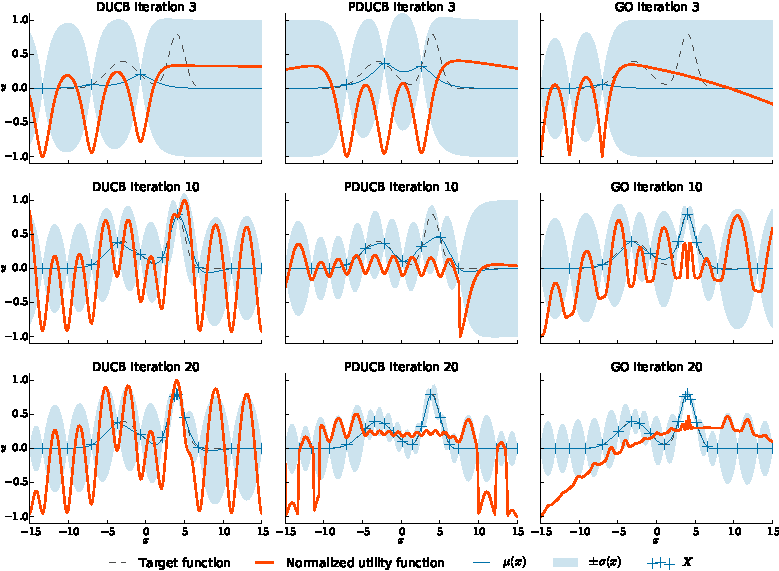
\includegraphics{plots/acqfns}
    \caption{TODO blab lorem ipsum}
\end{figure}

% TODO 1d example


\chapter{TODO}
- concrete scenarios
- error measures
- sampling
- discussion of implementation: Python, Numpy, Scipy, TCP protocol, QRSim, 
lbfgsb for optimization

\printbibliography

\end{document}
